\documentclass[11pt,a4paper]{article}
\usepackage[landscape,margin=0.5in]{geometry}
\usepackage{tikz}
\usetikzlibrary{shapes.geometric, arrows.meta, positioning, calc}
\pagestyle{empty}

\begin{document}
\begin{center}
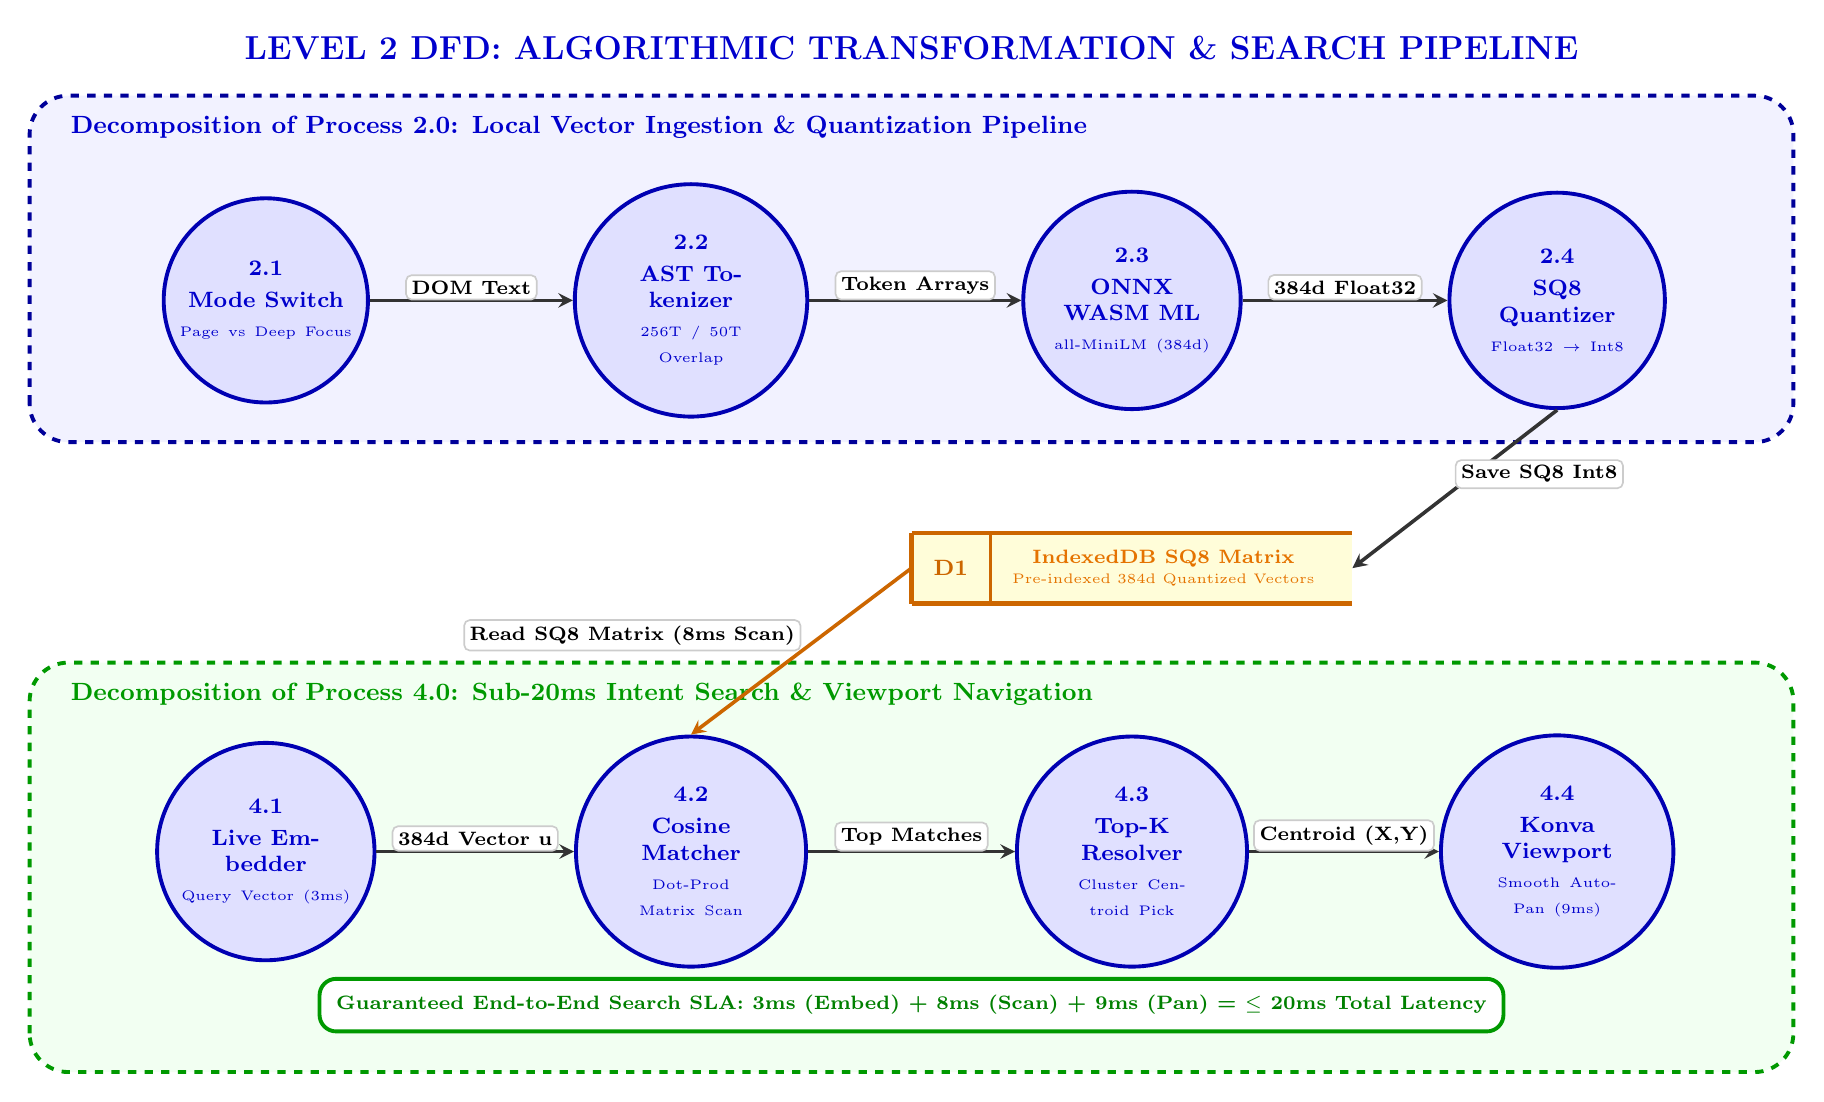
\begin{tikzpicture}[
    font=\sffamily,
    >=stealth,
    container1/.style={
        draw=blue!60!black, fill=blue!5, line width=1.4pt, dashed, rounded corners=14pt
    },
    container2/.style={
        draw=green!60!black, fill=green!5, line width=1.4pt, dashed, rounded corners=14pt
    },
    subproc/.style={
        circle, draw=blue!70!black, fill=blue!12, line width=1.4pt,
        text width=2.2cm, align=center, inner sep=2pt, font=\footnotesize\bfseries, text=blue!80!black
    },
    flow/.style={
        ->, >=stealth, line width=1.3pt, draw=black!80
    },
    labelbox/.style={
        fill=white, draw=gray!40, line width=0.6pt, rounded corners=2pt,
        inner sep=2pt, font=\scriptsize\bfseries, text=black
    }
]

    % Title
    \node[font=\large\bfseries, text=blue!80!black] at (0, 6.4) {LEVEL 2 DFD: ALGORITHMIC TRANSFORMATION \& SEARCH PIPELINE};

    % Container 1: Process 2.0 Breakdown
    \draw[container1] (-11.2, 1.4) rectangle (11.2, 5.8);
    \node[anchor=west, font=\small\bfseries, text=blue!80!black] at (-10.8, 5.4) {Decomposition of Process 2.0: Local Vector Ingestion \& Quantization Pipeline};

    % Container 2: Process 4.0 Breakdown
    \draw[container2] (-11.2, -6.6) rectangle (11.2, -1.4);
    \node[anchor=west, font=\small\bfseries, text=green!60!black] at (-10.8, -1.8) {Decomposition of Process 4.0: Sub-20ms Intent Search \& Viewport Navigation};

    % Top Row Subprocesses
    \node[subproc] (sp21) at (-8.2, 3.2) {2.1\\[2pt]Mode Switch\\[1pt]\tiny\normalfont Page vs Deep Focus};
    \node[subproc] (sp22) at (-2.8, 3.2) {2.2\\[2pt]AST Tokenizer\\[1pt]\tiny\normalfont 256T / 50T Overlap};
    \node[subproc] (sp23) at (2.8, 3.2) {2.3\\[2pt]ONNX WASM ML\\[1pt]\tiny\normalfont all-MiniLM (384d)};
    \node[subproc] (sp24) at (8.2, 3.2) {2.4\\[2pt]SQ8 Quantizer\\[1pt]\tiny\normalfont Float32 $\to$ Int8};

    % Bottom Row Subprocesses
    \node[subproc] (sp41) at (-8.2, -3.8) {4.1\\[2pt]Live Embedder\\[1pt]\tiny\normalfont Query Vector (3ms)};
    \node[subproc] (sp42) at (-2.8, -3.8) {4.2\\[2pt]Cosine Matcher\\[1pt]\tiny\normalfont Dot-Prod Matrix Scan};
    \node[subproc] (sp43) at (2.8, -3.8) {4.3\\[2pt]Top-K Resolver\\[1pt]\tiny\normalfont Cluster Centroid Pick};
    \node[subproc] (sp44) at (8.2, -3.8) {4.4\\[2pt]Konva Viewport\\[1pt]\tiny\normalfont Smooth Auto-Pan (9ms)};

    % Center Data Store D1
    \begin{scope}[shift={(2.8, -0.2)}]
        \fill[yellow!15] (-2.8, -0.45) rectangle (2.8, 0.45);
        \draw[line width=1.5pt, draw=orange!80!black] (-2.8, 0.45) -- (2.8, 0.45);
        \draw[line width=1.5pt, draw=orange!80!black] (-2.8, -0.45) -- (2.8, -0.45);
        \draw[line width=1.5pt, draw=orange!80!black] (-2.8, -0.45) -- (-2.8, 0.45);
        \draw[line width=1.0pt, draw=orange!80!black] (-1.8, -0.45) -- (-1.8, 0.45);
        \node[font=\footnotesize\bfseries, text=orange!80!black] at (-2.3, 0) {D1};
        \node[align=center, font=\scriptsize\bfseries, text=orange!90!black] at (0.4, 0) {IndexedDB SQ8 Matrix\\[-1pt]\tiny\normalfont Pre-indexed 384d Quantized Vectors};
        \coordinate (d1_east) at (2.8, 0);
        \coordinate (d1_west) at (-2.8, 0);
    \end{scope}

    % Top Row Connections
    \draw[flow] (sp21.east) -- (sp22.west) node[midway, above, labelbox] {DOM Text};
    \draw[flow] (sp22.east) -- (sp23.west) node[midway, above, labelbox] {Token Arrays};
    \draw[flow] (sp23.east) -- (sp24.west) node[midway, above, labelbox] {384d Float32};
    \draw[flow] (sp24.south) -- (d1_east) node[midway, above right, labelbox] {Save SQ8 Int8};

    % D1 to Bottom Row Connection
    \draw[flow, draw=orange!80!black] (d1_west) -- (sp42.north) node[midway, above left, labelbox] {Read SQ8 Matrix (8ms Scan)};

    % Bottom Row Connections
    \draw[flow] (sp41.east) -- (sp42.west) node[midway, above, labelbox] {384d Vector u};
    \draw[flow] (sp42.east) -- (sp43.west) node[midway, above, labelbox] {Top Matches};
    \draw[flow] (sp43.east) -- (sp44.west) node[midway, above, labelbox] {Centroid (X,Y)};

    % Bottom SLA Banner
    \node[draw=green!60!black, fill=white, line width=1.4pt, rounded corners=6pt,
          inner sep=6pt, font=\scriptsize\bfseries, text=green!50!black] at (0, -5.75)
          {Guaranteed End-to-End Search SLA: 3ms (Embed) + 8ms (Scan) + 9ms (Pan) = $\le$ 20ms Total Latency};

\end{tikzpicture}
\end{center}
\end{document}